%Architecture montrant le découpage des différents modules logiciels et matériels et leurs interactions dynamiques (diagramme UML : composants, déploiement, séquence)
%Spécification d'interface entre les composants
%Sécurité


\subsection{Architecture Globale}
De façon globale, on peut voir le système final comme l'assemblage de 3 grands modules, eux mêmes composés de sous modules. 

Notre POC est composé des modules suivants:
\begin{itemize}
	\item Extraction du texte brut
	\item Extraction de métadonnées
	\item Recherche des taxonomies
	\item Moteur de recherche
\end{itemize}

Ce choix de considérer le projet comme un ensemble de modules interagissants les uns avec les autres plutôt que comme un monolithe nous a permis une plus grande flexibilité de développement, ainsi qu'une meilleure testabilité.
En effet le développement de chaque modules peut ainsi être réalisé en parallèle.
Cette répartition du travail nous permet également de faire une liste des objectifs de développement plus précise. 

Ces modules sont indépendants des uns des autres, dans le sens où il ne partageront que des fichiers entre eux.

En effet, le but du premier module est d'extraire le texte des fichiers PDF\@.
Ce texte est ensuite la base sur laquelle les modules d'extraction de métadonnées et de taxonomies pourront travailler.
Ces modules sont appelés par un programme de création de fichier \gls{JSON}, fichier qui sera finalement utilisé par le module `Moteur de recherche'. 

Il était donc important de s'accorder précisément sur le format de sortie de chaque modules pour assurer la compatibilité entre les modules.

\subsection{Extraction du texte brut}
La majorité des documents que nous avons pu obtenir sont au format PDF\@.
Ce format est portable, et est très couramment utilisé pour sa simplicité et son poids assez faible.

Pour pouvoir analyser correctement ces documents, nous devons extraire le texte inclus dans ces fichiers.
Ce texte sera ensuite utilisé pour l'extraction des métadonnées et l'ajout de termes taxonomiques.
Selon la façon dont le fichier a été enregistré, et les objets contenus (tableaux, images), la qualité de l'extraction du texte peut fortement varier. 

Nous utilisons une approche double, qui nous assure une haute qualité d'extraction avec un temps d'exécution raisonnable.
A l'aide d'un script bash, nous listons tous les fichiers disponibles dans le dossier initial donné par l'utilisateur. 

Nous utilisons d'abord un utilitaire appelé `pdftotext' qui tente une extraction simple en analysant le fichier PDF pour en sortir le texte inscrit.
Il se peut cependant que cette approche ne donne pas de résultat, si le document est une suite d'images scannées par exemple.

Dans ce cas, nous avons développé une approche basé sur Tesseract\cite{tess}, un programme d'\gls{ocr} (Optical Character Recognition) développé en parti par Google. 

L'OCR tente d'extraire du texte caractères par caractères depuis une image.
Les techniques actuelles se basent sur des modèles de Deep Learning tels que le \glspl{lstm} et les \glspl{cnn}, qui vont essayer de localiser les zones de texte et d'en tirer les caractères présents.
Cette approche, bien que souvent efficace, peut également faillir, et donner en sortie des caractères erronés.
La qualité du texte extrait étant critique pour le reste du projet, beaucoup de soins ont été donnés dans le prétraitement du fichier PDF image pour obtenir une qualité d'extraction optimale.

\begin{figure}[h!]
  \centering
	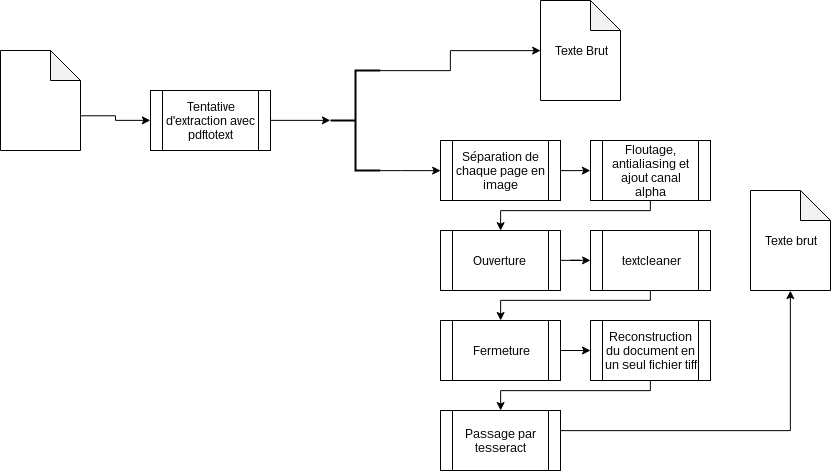
\includegraphics[width=0.7\textwidth]{extractionText.png}
	\caption[]{Diagramme fonctionnel du module d'extraction du texte}
  \label{}
\end{figure}


\subsection{Extraction des métadonnées}
Les métadonnées sont des informations \textit{concernant} le document.
Nous avons choisi de construire des fonctions spécialisées, chacune ayant pour rôle d'extraire un type de métadonnée particulière.
Cette spécialisation nous permet de facilement ajouter des types de métadonnées à la sortie finale et respecte une volonté de compartimentalisation des responsabilités du programme: pour chaque type d'information à extraire du texte, i.e\. taxonomie, numéro d'article, date de publication, une fonction lui est dédié. 
Cela nous permet d'effectuer des corrections spécifiques a chaque données.

Pour le cas de la taxonomie, le schéma global de fonctionnement est le suivant: une fonction d'ajout de métadonnées au fichier JSON appelle chaque fonctions d'extraction individuellement.
La figure~\ref{fig:globalMeta} représente un diagramme fonctionnel général de l'extraction de métadonnées. 
Ces fonctions sont généralement courtes et consistent de RegEx spécialement construites pour extraire l'information demandée.
Pour rappel, une RegEx est une séquence de caractères définissant un schéma de recherche précis.
Ces fonctions ont l'avantage d'être extrêmement rapides, avec un temps d'exécution de quelques millisecondes, même pour des documents comportant des centaines de pages. 

\begin{figure}[h!]
  \centering
	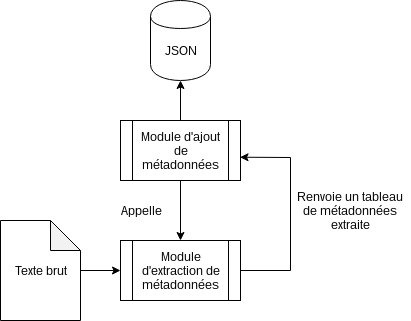
\includegraphics[width=0.5\textwidth]{SchemaGlobal.png}
	\caption[]{Diagramme fonctionnel général des fonctions permettant l'extraction des métadonnées}
  \label{fig:globalMeta}
\end{figure}

Chacune de ces fonctions prends en entrée le texte brut traité pour en enlever les accents et caractères spéciaux, et ressort un tableau comportant les métadonnées extraites.
Ces tableaux sont directement insérées dans le fichier JSON, qui constitue la base sur lequel le moteur de recherche fonctionne.


\subsection{Module taxonomique}

\begin{figure}[h!]
  \centering
  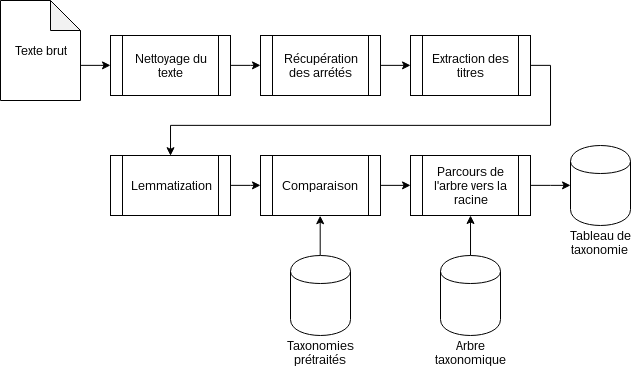
\includegraphics[width=0.8\textwidth]{diagArchiTaxo.png}
	\caption[]{Diagramme de l'architecture du module taxonomique}
  \label{}
\end{figure}

Le module taxonomique à pour charge d'extraire et d'assigner un ou plusieurs termes taxonomiques à un document.

Pour des raisons d'efficacité et de précision que nous détaillerons en sous-section~\ref{word2vecReal}, ce module extrait d'abord les titres des arrêtés contenus dans le texte, puis les compare avec les taxonomies après une normalisation.

Cette normalisation consiste en une lemmatisation, procédure où l'on remplace un mot par sa racine.
Ces opérations permettent une comparaison plus robuste et moins dépendante du contexte de la phrase. 

\begin{figure}[h!]
  \centering
  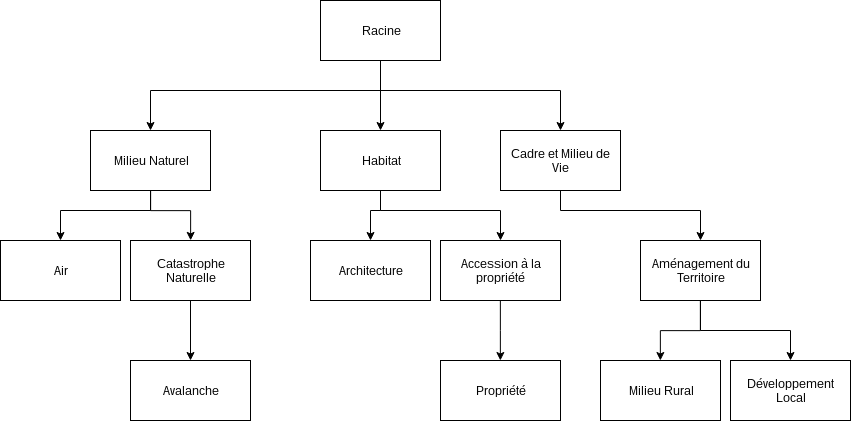
\includegraphics[width=0.8\textwidth]{TaxoTree.png}
	\caption[]{Aperçu de l'arbre taxonomique}
  \label{fig:tree}
\end{figure}

Pour chaque termes de la taxonomie, le module va vérifier si celui ci est présent dans le titre qu'il est en train d'analyser.
Si oui, ce terme est ajouté à un tableau contenant les taxonomies du document, ainsi que tous ses parents de l'arbre taxonomique.


\subsection{Moteur de recherche avec Reactivesearch/Appbase.io}
Appbase est le site qui va centraliser l'ensemble des données et les rendre visibles à travers une interface.
Le module moteur de recherche fonctionne indépendamment des autres modules. Une fois les métadonnées et la taxonomie importés dans le format JSON, ElasticSearch effectue l'indexation.
Avec Reactivesearch il existe plusieurs modules tels que les champs de recherche avec l'autosuggestion ou l'ajout des filtres.  

Afin d'importer nos données, nous devons respecter le format JSON\@.
Dans un premier temps, nous créons une application depuis Appbase.io. 
Un JSON se compose de plusieurs documents où chaque document est enlacé par des accolades.
Dans un document, nous avons des champs qui correspondent aux différentes familles de données récoltés.
Dans notre cas, nous avons comme exemple de champs les noms, les arrêtés ou les numéros de recueils.

La structure du JSON pour ElasticSearch est la suivante :
\begin{lstlisting}
	{
		"field": "value",
		"index": 1
	},
	{
		"RAA": {"ref du RAA"},
		"dates": {"2017-07-25", ...},
		...
	},
	...
\end{lstlisting}

Cette structure est différente pour Reactivesearch :
\begin{lstlisting}
[
	{
		"RAA": {"ref du RAA"},
		"dates": {"2017-07-25", ...},
		...
	}, 
	...
]
\end{lstlisting}

Lorsque les données sont correctement importées un mail est envoyé contenant le "credentials" (identifiant) afin de spécifier l'accessibilité aux données.
Les données sont alors affichées en ligne sur le site internet.
Cela nous permet de visualiser ce qui a été importé. 

\begin{figure}[h!]
  \centering
	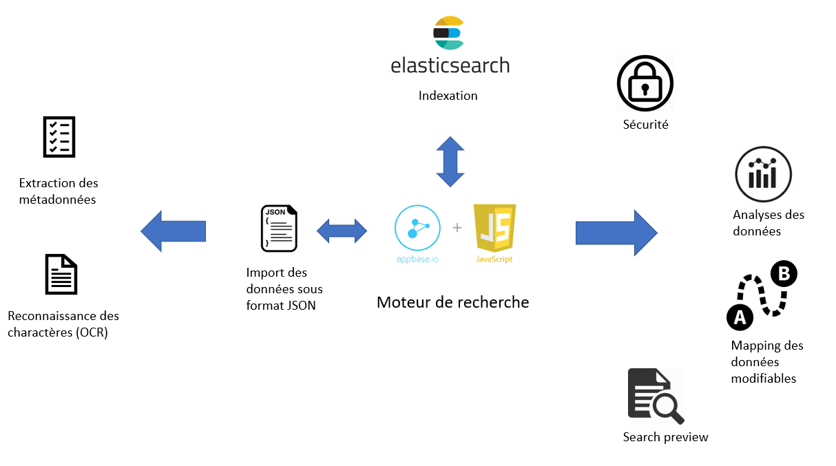
\includegraphics[width=0.7\textwidth]{SpecTechArchiMoteur.png}
	\caption[]{Diagramme fonctionnel du moteur de recherche}
  \label{}
\end{figure}

Le résultat des recherches s'affichent sous la forme d'une suite de cartes composés chacune d’un titre, d’une description et d’une URL\@.
La description contient la date de publication du document et les 4 termes taxonomiques les plus pertinents.

Nous avons également ajouté des filtres de recherche qui permettent de réduire le cadre de recherche pour obtenir des résultat plus précis.

CodesSandbox permet d’avoir accès au code Javascript généré par Appbase.io.
Ce dernier a la particularité d’être multiplateformes et de nous donner accès un lien d’accès web vers l'application.
Notre moteur de recherche est donc accessible en ligne.
